\documentclass{article}
\usepackage{mystyle}
\usepackage{float}
\usepackage{enumitem}
\usepackage{amsthm}
\usepackage{amsmath}
\usepackage{amssymb}
\usepackage{graphicx}
\usepackage[colorlinks = true, linkcolor = blue, urlcolor = cyan]{hyperref}

\theoremstyle{definition}
\newtheorem{theorem}{Theorem}[section]
\newtheorem{lem}{Lemma}[section]
\newtheorem{cor}{Corollary}[theorem]
\newtheorem{defn}{Definition}[section]
\newtheorem{prop}{Proposition}[section]
\newtheorem{ax}{Axiom}[section]
\newtheorem{example}{Example}[section]

\title{Mechanism Design}
\author{
	\textbf{Raj Aryan Agrawal}\\
	190050097\\
	Undergraduate, Department of Computer Science\\
	Indian Institute of Technology Bombay
}


\begin{document}
\maketitle
\setcounter{tocdepth}{2}
\tableofcontents

\section{Introduction}
Mechanism design is concerned with settings where a policy maker faces the problem of aggregating the \textit{announced preferences} of players into a system wide decision when the \textit{actual preferences} of the players are not publicly known. That is we need to solve an optimization problem with incomplete information.\\
Mechanism design uses a technique that induces a game among the agents such that the equilibrium of the induced game - the desired system wide solution is implemented.
\subsection{Cake Cutting Problem}
\begin{example}
\textbf{(Cake Cutting Problem)} Consider the mother of 2 kids, who has to design a mechanism to make her kids share a cake equally. Here the mother is the social planner (policy maker). If the mother slices the cake into 2 equal pieces and distributes, this may not be an acceptable solution as each kid will have the perception he got the smaller piece.\\
Instead consider the mechanism
\begin{itemize}
	\item One of the kids would slice the cake into 2 pieces
	\item The other kid gets the chance to pick up any of the pieces and leaves the other for first
\end{itemize}
Child $1$ will slice cake into 2 equal halves (in \textit{his} eyes), as any other division will leave him with a smaller piece as the remaining piece.\\
Child $2$ is happy because he gets to choose and so will choose what appears larger among the 2 in \textit{his} eyes.\\
Thus this mechanism gives desired outcome and both agents are happy.
\end{example}
\subsubsection{Generalised Cake Cutting}
This is a mechanism for $n$ players dividing a cake. We say an allocation is \textit{fair} if $u_i(piece_i) \geq 1/n$ for each player and envy-free if $u_i(piece_i)\geq u_i(piece_j)$ for each $i$ and $j$. Then the algorithm is - \\
\textbf{Banach - Knaster Discrete Protocol}
\begin{itemize}
	\item A player cuts a piece which he believes to be size $1/n$
	\item Every other player can trim the piece to what they consider $1/n$ or pass if they believe it is size $1/n$
	\item Last player to cut the piece gets to keep it
\end{itemize}
This method will give a fair and envy free distribution. In a round, in the eyes of all players the piece is of size $1/n$ at their round and any subsequent trimming is only reducing the size. For the last player (recieving player), the size of cake is exactly $1/n$, hence it is fair. 
\subsection{Social Choice Function}
\begin{defn}
\textbf{(Mechanism Design Setting)} We define the setting as 
\begin{itemize}
	\item $N = \{1,2,\dots,n\}$ is the set of agents which are all rational and intelligent.
	\item $X$ is the set of possible outcomes. Agents decide a collective choice from the set $X$
	\item Before making a collective choice, each agent privately observes his preferences over alternatives in $X$. This is modelled by supposing each agent $i$ has a private value $\theta_i$ that determines his preferences and is private to player $i$
	\item $\Theta_i$ is the set of private values for agent $i$ and $\Theta = \Theta_1\times\dots\times\Theta_n$ os set of all type profiles.
	\item $\mathbb{P}\in \Delta(\Theta)$ is a common prior. To ensure consistency of beliefs, individual belief functions $p_i:\Theta_i \mapsto \Delta(\Theta_{-i})$ can be all derived from common prior.
	\item Individual agents have preferences over the outcomes represented by utility function $u_i : X\times \Theta_i \mapsto \mathbb{R}$. Given $x\in X$ and $\theta_i \in \Theta_i$ the value $u_i(x,\theta_i)$ is the payoff for agent $i$. $u_i$ can depend on types of other players as well, where $u_i: X\times \Theta \mapsto \mathbb{R}$.
	\item $X,N,\Theta_i,\mathbb{P}$ and $u_i$ are assumed to be common knowledge among all players. The specific type $\theta_i$ is private information.
\end{itemize}
\end{defn}

\begin{defn}
\textbf{(Social Choice Function)} Suppose $N = \{1,\dots,n\}$ is a set of agents with type sets $\Theta_i$ for each $i$. given a set of outcomes $X$, a social choice function is a mapping $f:\Theta \mapsto X$. The outcome corresponding to a type profile is called the social choice.
\end{defn}
Consider a social choice function $f:\Theta \mapsto X$, the types $\theta_i$ are private information.
\begin{defn}
\textbf{(Preferance Elicitation Problem)} For the social choice $f(\theta_1,\dots,\theta_n)$ to be chosen when individual types are $\theta_i$ each agent must disclose true type to social planner. But all agents may not find it a best interest to reveal this. This is the \textit{information relevation problem}
\end{defn}
\begin{defn}
\textbf{(Preference Aggregation Problem)} On obtaining all the reported types, suppose $\theta_i$ is the true type and $\hat{\theta_i}$ is the reported type, then process of computing $f(\hat{\theta_1},\dots,\hat{\theta_n})$ is called the preference aggregation problem.
\end{defn}
\begin{figure}[H]
\centering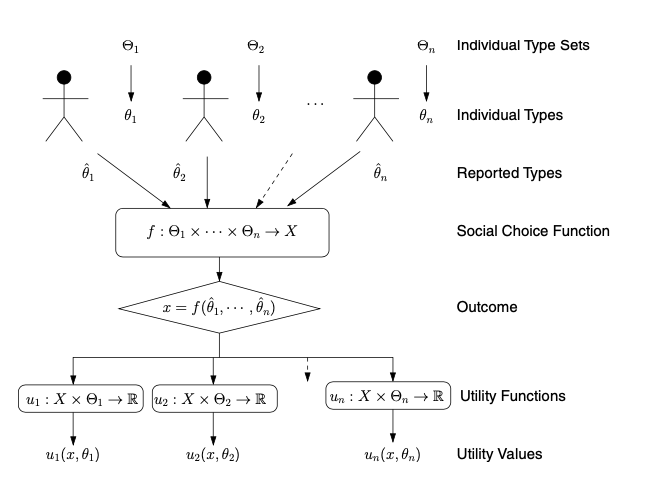
\includegraphics[scale = 0.3]{images/Fig3.png}
\caption{Mechanism Design Environment}
\end{figure}
\begin{example}
\textbf{(Selling an Indivisible Object)} Suppose there is 1 seller and $n$ buyers, let sellet be agent $0$ and the $n$ buyers be ordered $1,2,\dots,n$, hence $N = \{0,1,\dots,n\}$. Then we can define the allocation $$X = \{(y_0,y_1,\dots,y_n,t_0,t_1,\dots,t_n)| y_i \in \{0,1\}; \sum_{i=0}^n y_i = 1; t_i \in R; i \in N\}$$ where $y_i$ takes 1 if object allocated to player $i$ and $0$ otherwise. $t_i$ is the payment received by agent $i$. For $x \in X$, we can define utility in a natural way as $u_i(x,\theta_i) = y_i\theta_i + t_i$, where $\theta_i \in \mathbb{R}_+$ can be viewed as agent $i$'s valutation of the object. Such utility functions are called \textit{quasi linear} as they are linear in some variables and possible non linear in other. Now we assume 
\begin{itemize}
	\item Seller has a known value $\theta_0$, that is $\Theta_0 = \{\theta_0\}$
	\item $\Theta_i \subseteq \mathbb{R}_+$ is the set of all possible evaluations of buyer $i$, this can be viewed as the willingness to pay (above which buyer is not interested in paying)
\end{itemize}
Consider the Social Choice function
\begin{itemize}
	\item Selling agent allocates the object to buyer with highest willingness to buy, in case multiple buyers, it is given to the agent with smallest $i$
	\item The allocated buyer $i$ pays amount $\theta_i$ to selling agent.
\end{itemize}
Then the social choice function is $f(\theta) = \{y_0(\theta),\dots,y_n(\theta),t_0(\theta),\dots,t_n(\theta))$ which is 
$$y_0 = 0$$
$$y_i(\theta) = 
\begin{cases}
1 & \text{ if } \theta_i > \theta_j~\forall j<i; ~ \theta_i\geq \theta_j ~\forall j>i;~i,j \in \{1,2,\dots,n\}\\
0 & \text{ otherwise }
\end{cases}$$
$$t_i(\theta) = -y_i(\theta)\theta_i~\forall i \in \{1,\dots,n\}$$
$$t_0(\theta) = -\sum_{i=1}^n t_i(\theta)$$
\end{example}
\section{Implementation of Social Choice Functions by Mechanisms}
Mechanism design is an optimization problem where the specifications are first elicited and then the decision problem is solved. To elicit the type information in a truthful way there are 2 main approaches.
\begin{defn}
\textbf{(Direct Mechanism)} Suppose $f:\Theta\mapsto X$ is a social choice function. A direct mechanism (\textit{direct revelation mechaism}) is the tuple $(\Theta_1,\dots,\Theta_n,f(.))$
\end{defn}
That is we directly seek the type information from agents by asking them to reveal their true types.
\begin{defn}
\textbf{(Indirect Mechanism)} An indirect mechanism consists of a tuple $(S_1,\dots,S_n, g(.))$ where $S_i$ is a set of possible actions for agent $i$ and $g: S_1\times \dots\times S_n \mapsto X$ is a function that maps each action profile to an outcome.
\end{defn}
The idea is we induce a game among the players and the strategies played at equilibrium of this game will indirectly reflect their original types. The direct mechanism is a speical case of an indirect mechanism.
\subsection{Implementation by Direct Mechanism}
\end{document}